%%%%%%%%%%%%%%%%%%%%%%%%%%%%%%%%%%%%%%%%%%%%%%%%%%%%%%%%%%%
%%
%% MARK: Chapter 2 — The Prequantum Groupoid for Simply Connected Spaces
%%
%%%%%%%%%%%%%%%%%%%%%%%%%%%%%%%%%%%%%%%%%%%%%%%%%%%%%%%%%%%
\chapter{The Prequantum Groupoid for Simply Connected Spaces}
\label{chap:The Prequantum Groupoid for Simply Connected Spaces}

In this chapter,
we construct the \emph{prequantum groupoid} $\Groupoid{T}_\omega$ for a connected and simply connected parasymplectic space $(X,\omega)$.
The construction proceeds by distilling the space of paths $\Paths(X)$,
equipped with its canonical \emph{paths-primitive} $1$-form $\Komega$,
into a diffeological groupoid $\Groupoid{T}_\omega$ whose space of morphisms is the quotient $\cY = \Paths(X)/\!\sim_\omega$.
The equivalence relation $\sim_\omega$ identifies paths that have the same endpoints and whose relative symplectic action belongs to the group of periods $\Pomega$.
The resulting groupoid carries a canonical left-right invariant $1$-form $\blambda$,
called the \emph{prequantum $1$-form},
whose curvature encodes the classical form $\omega$.
We show that the isotropy group of $\Groupoid{T}_\omega$ at any point is isomorphic to the torus of periods $\Tomega = \fieldR/\Pomega$,
and that the full symmetry group $\Diff(X,\omega)$ lifts faithfully to automorphisms of $(\Groupoid{T}_\omega,\blambda)$.
This chapter establishes the foundations of the Geometric Quantization by Paths (GQbP) framework
in the simplest geometrical setting,
paving the way for the generalizations to come.

%%%%%%%%%%%%%%%%%%%%%%%%%%%%%%%%%%%%%%%%%%%%%%%%%%%%%%%%%%%
%%
%% MARK: Section — Parasymplectic spaces and the group of periods
%%
%%%%%%%%%%%%%%%%%%%%%%%%%%%%%%%%%%%%%%%%%%%%%%%%%%%%%%%%%%%
\section{Parasymplectic Spaces and the Group of Periods}
\label{sec:Parasymplectic Spaces and the Group of Periods}

In this section,
we introduce the classical data of the system:
a connected and simply connected diffeological space $X$ equipped with a closed $2$-form $\omega$.
We call such a pair $(X,\omega)$ a \emph{parasymplectic space}
(the space $X$ need not be simply connected for this definition to make sense).
We use the term ``parasymplectic'' because $\omega$ is not required to be symplectic
(no non-degeneracy condition is imposed)
nor presymplectic (no constant rank condition is required).
The notion of symplectic form in diffeology remains a subject of discussion,
as different formal definitions have been proposed
(see the discussion in \cite{PIZ10}).
However,
as we shall see,
this condition has no impact on the geometric quantization by paths
for the construction of a general quantum system associated with a diffeological space equipped with a closed $2$-form.

From this classical data,
we construct the canonical \emph{paths-primitive} $1$-form $\Komega$ on the space of paths $\Paths(X)$,
that is,
$\Komega \in\DForms^1(\Paths(X))$.
For $X$ connected and simply connected,
we define its \emph{group of periods} $\Pomega \subset \fieldR$.
In this case,
the condition $\Pomega \neq \fieldR$ (discreteness of the periods)
is the necessary and sufficient condition for the existence of the prequantum groupoid.
It leads to the \emph{torus of periods} $\Tomega = \fieldR/\Pomega$,
which will later emerge as the isotropy group of the quantum system
and as the geometric origin of the \emph{quantum phase}.

%%%%%%%%%%%%%%%%%%%%%%%%%%%%%%%%%%%%%%%%%%%%%%%%%%%%%%%%%%%
%% MARK: Article — The Classical Data
%%%%%%%%%%%%%%%%%%%%%%%%%%%%%%%%%%%%%%%%%%%%%%%%%%%%%%%%%%%
\begin{article}\artlabel[The Classical Data]
  \label{art:classical-data}
  Let $X$ be a diffeological space.
  We assume that $X$ is \emph{connected} and \emph{simply connected}:
  any two points can be joined by a smooth path,
  and every smooth loop is homotopic to a constant path.
  These assumptions simplify the construction that follows,
  and will be removed in the next chapter.
  
  Let $\omega \in \DForms^2(X)$ be a closed $2$-form,
  \ie,
  $\der\omega = 0$.
  We call the pair $(X,\omega)$ a \emph{parasymplectic space}.
  The term emphasizes that we impose no non-degeneracy condition on $\omega$:
  $\omega$ need not be symplectic (``non-degenerate'' in some sense) nor presymplectic (``constant rank'').
  The precise notions of symplectic and presymplectic in diffeology are discussed in \cite{PIZ10}.%
  \footnote{A diffeological $2$-form would be presymplectic if its automorphism group $\Diff(X,\omega)$ acts locally transitively,
  and symplectic if the universal $1$-point moment map $\mu_\omega$ (with respect to the automorphism group) is injective.
  This last condition may be refined in the future.
  In any case,
  these notions are irrelevant to the construction presented here,
  which is part of its interest.}
  As we shall see,
  geometric quantization by paths requires no such regularity.
  It works for any closed $2$-form,
  regardless of degeneracies or singularities of the underlying space.
  
  The case $\omega = 0$ is not excluded,
  but we will momentarily set it aside.
  It leads to the pair groupoid $X \times X$ with vanishing prequantum $1$-form,
  which will later appear as the neutral element in the abelian group structure
  of isomorphism classes of prequantum groupoids
  (a structure to be discussed in a later chapter).
\end{article}

%%%%%%%%%%%%%%%%%%%%%%%%%%%%%%%%%%%%%%%%%%%%%%%%%%%%%%%%%%%
%% MARK:  Article — The Paths-Primitives
%%%%%%%%%%%%%%%%%%%%%%%%%%%%%%%%%%%%%%%%%%%%%%%%%%%%%%%%%%%
\begin{article}\artlabel[The Paths-Primitives]
  \label{art:paths-primitives}
  Recall from the Primer (Chapter~I, \S\ref{subsec:The Chain-Homotopy Operator})
  the chain-homotopy operator
  \[
    \CHO: \DForms^k(X) \to \DForms^{k-1}(\Paths(X)).
    \]%
  This operator is \emph{canonical}:
  it requires no choice.
  It is defined purely in terms of the smooth structure of $X$ and $\Paths(X)$.
  
  For any closed $k$-form $\beta \in \DForms^k(X)$,
  applying $\CHO$ and using $\der\beta = 0$,
  by the chain-homotopy identity $\der \circ \CHO + \CHO \circ \der = \1^* - \0^*$,
  we obtain the $(k-1)$-form
  \[
    \Kbeta \in \DForms^{k-1}(\Paths(X)),
    \qtext{satisfying:}
    \der[\Kbeta] = \1^*\beta - \0^*\beta.
    \]%
  The maps $\0, \1: \Paths(X) \to X$ are the source and target maps
  $\1(\gamma) = \gamma(1)$ and $\0(\gamma) = \gamma(0)$.
  
  \begin{definition}
    We call $\Kbeta$ the \emph{paths-primitive} of $\beta$.
  \end{definition}
  
  This terminology distinguishes $\Kbeta$ from the classical notion of \emph{transgression},
  which operates on cohomology classes and requires choices at every step.
  The paths-primitive is a genuine differential form on the infinite-dimensional space $\Paths(X)$,
  well-defined within the diffeological framework.
  
  \begin{proposition}
    The chain-homotopy operator $\CHO$ is injective on closed forms.
    That is,
    if $\beta \in \DForms^k(X)$ is closed and $\Kbeta = 0$,
    then $\beta = 0$.
    In symbols,
    \[
      \ker(\CHO \restriction \ZDR^*(X)) = \{0\}.
      \]%
  \end{proposition}
  
  This injectivity guarantees that the passage from $\beta$ to $\Kbeta$ loses no information:
  the paths-primitive faithfully encodes the original closed form.
  This property is crucial for the geometric quantization by paths which is the subject of this memoir,
  because it ensures that the passage from the classical parasymplectic form $\omega \in \ZDR^2(X)$
  to its paths-primitive $\Komega \in \DForms^1(\Paths(X))$
  retains all the information encoded in $\omega$.
\end{article}

\begin{proof}
  Assume $\Kbeta = 0$.
  Applying the exterior derivative,
  we obtain $\der\Kbeta = 0$.
  But the chain-homotopy identity gives $\der\Kbeta = \1^*\beta - \0^*\beta$,
  hence $\1^*\beta - \0^*\beta = 0$ on $\Paths(X)$.
  Restrict to the subspace $\Paths(X,x,\ast)$ of paths with source $x$,
  for any point $x \in X$.
  On this subspace $\0^*\beta = 0$ (since $\0$ is the constant map $\gamma \mapsto x$),
  so the identity reduces to $\1^*(\beta) = 0$.
  Since $X$ is connected,
  the target map $\1: \Paths(X,x,\ast) \to X$ is a subduction
  \cite[\textsection 5.6]{PIZ13},
  and a subduction pulling back a form to zero forces that form to vanish
  \cite[\textsection 6.39]{PIZ13}.
  Therefore $\beta = 0$.
\end{proof}

%%%%%%%%%%%%%%%%%%%%%%%%%%%%%%%%%%%%%%%%%%%%%%%%%%%%%%%%%%%
%% MARK:  Article — Integration of Closed $1$-forms
%%%%%%%%%%%%%%%%%%%%%%%%%%%%%%%%%%%%%%%%%%%%%%%%%%%%%%%%%%%
\begin{article}\artlabel[Integration of Closed $1$-forms]
  \label{art: Integration of Closed 1-forms}
  The first application of the chain-homotopy operator $\CHO$ is the
  \emph{integration of a closed $1$-form}.
  We recall the classical case of a manifold $M$ and a closed $1$-form $\alpha$ on $M$
  with discrete periods $P_\alpha = a \ZZ \subset \fieldR$,
  the group of integrals of $\alpha$ over loops in $M$.
  For such a form,
  there exists a function $f$, defined up to an additive constant, by
  \[
    f(x) = \int_\gamma \alpha \mod a,
    \widetext{or equivalently, if $a \neq 0$,}
    f(x) = e^{\frac{2\pi i}{a}\int_\gamma \alpha},
    \]%
  where $\gamma$ is any path in $M$ from a fixed origin $o$ to $x$,
  that is, $\gamma(0) = o$ and $\gamma(1) = x$.
  In the first formulation $\alpha = \der f$;
  in the second $\alpha = \frac{a}{2\pi i}\frac{\der f}{f}$.
  Choosing a different path changes the integral by an element of $P_\alpha$,
  which is absorbed by the quotient or by periodicity.
  
  This familiar construction is a particular case of a more general
  diffeological statement.
  Let $X$ be any connected diffeological space and let $\alpha$ be a closed $1$-form:
  \[
    \alpha \in \DForms^1(X),
    \quad
    \der\alpha = 0.
    \]%
  The chain homotopy operator applied to $\alpha$ yields a $0$-form $\Kalpha \in \DForms^0(\Paths(X))$,
  which we will call the \emph{path primitive} of $\alpha$.
  \[
    \Kalpha \in \Cinfty(\Paths(X),\fieldR),
    \widetext{with}
    \Kalpha(\gamma) = \int_\gamma \alpha := \int_0^1 \alpha(\gamma)_t(1)\, \dt.
    \]%
  
  \begin{definition}
    Let $\alpha$ be a closed $1$-form on a connected diffeological space $X$.
    The \emph{group of periods} of $\alpha$ is
    \[
      \Periods_\alpha = \left\{ \int_\ell \alpha \;\Big|\; \ell \in \Loops(X) \right\}.
      \]%
  \end{definition}
  
  \begin{proposition}[1]
    The set $\Periods_\alpha$ is a subgroup of $\fieldR$.
    If $\Periods_\alpha$ is discrete in the diffeological sense,%
    \footnote{A subgroup of a diffeological group is discrete if it inherits the
    discrete diffeology by restriction,
    which for a subgroup of $\fieldR$ is equivalent to $\Periods_\alpha \neq \fieldR$.
    See the Primer, \S\ref{art:One-Dimensional Tori}.}
    then the \emph{torus of periods}
    \[
      \Torus_\alpha = \fieldR/\Periods_\alpha
      \]%
    is a one-dimensional diffeological group.
    It carries a canonical invariant $1$-form $\theta$,
    defined by $\Proj_\alpha^*(\theta) = \dt$,
    where $\Proj_\alpha: \fieldR \to \Torus_\alpha$ is the canonical projection.
  \end{proposition}
  
  Consider now the smooth function $\Kalpha \in \Cinfty(\Paths(X),\fieldR)$.
  
  \begin{proposition}[2]
    The function $\Kalpha$ projects onto a smooth map
    $\phi: X \times X \to \Torus_\alpha$,
    called the \emph{$2$-point integration function},
    such that the following diagram commutes:
    \begin{center}
      \begin{tikzcd}[column sep=large, row sep=large]
        \Paths(X) \arrow[r,"\Kalpha"] \arrow[d, swap, "\EndsMap"] & \fieldR \arrow[d, "\Proj_\alpha"] \\
        X \times X \arrow[r, swap, "\phi"] & \Torus_\alpha
      \end{tikzcd}
    \end{center}
    It satisfies the following properties.
    \begin{enumerate}
      \item It is a \emph{Chasles cocycle}:
      for every three points $x,x',x'' \in X$,
      \[
        \phi(x,x') + \phi(x',x'') = \phi(x,x'').
        \]%
      \item It integrates the closed form $\alpha$ in the sense that
      \[
        \phi^*(\theta) + \alpha \ominus \alpha = 0,
        \]%
      where $\alpha \ominus \alpha$ is the $1$-form on $X \times X$ defined by
      $(\alpha \ominus \alpha)(P,Q) = \alpha(P) - \alpha(Q)$
      for every plot $(P,Q)$ in $X \times X$.
    \end{enumerate}
  \end{proposition}
  
  Since $X$ is connected and $\phi$ is a Chasles cocycle,
  the solutions $f$ of the equation $\phi(x,x') = f(x') - f(x)$
  are exactly the functions of the form
  \[
    f(x) = \phi(x_0,x) + \tau,
    \]%
  where $x_0 \in X$ is a chosen basepoint and $\tau \in \Torus_\alpha$ is an
  arbitrary constant.
  For any such solution,
  \[
    f^*(\theta) = \alpha.
    \]%
  We call these functions the \emph{integration functions} of $\alpha$.
  
  This construction generalizes the classical integration of a closed $1$-form
  on a manifold to the diffeological setting.
  The sole necessary condition is that the group of periods be
  diffeologically discrete.
\end{article}

\begin{proof}
  All loops and concatenations below are taken in the stationary sense,
  which does not affect the values of the integrals
  because $\alpha$ is closed and the de Rham integral is homotopy invariant.
  
  Let us begin by verifying that the set of periods of $\alpha$ is indeed a subgroup of $\fieldR$.
  The constant loop integrates to zero, so $0 \in \Periods_\alpha$.
  If $a,b \in \Periods_\alpha$ are the integrals of loops $\ell_a$ and $\ell_b$,
  conjugating $\ell_b$ to the basepoint of $\ell_a$ (which does not change
  its integral, since the homotopy swept out has zero area under $\der\alpha = 0$)
  and concatenating the two stationary loops
  gives a new loop whose integral is $a+b$.
  Reversing a loop changes the sign of the integral,
  so $-a \in \Periods_\alpha$.
  Hence $\Periods_\alpha$ is a subgroup of $\fieldR$.
  
  Then,
  we construct $\phi$ in three steps.
  
  \textbf{Step 1: Descent to the quotient.}
  Let $\gamma, \gamma' \in \Paths(X)$ be two paths with the same endpoints,
  $\EndsMap(\gamma) = \EndsMap(\gamma') = (x,x')$.
  The concatenation $\gamma' \vee \bar\gamma$ is a loop based at $x$,
  and
  \[
    \int_{\gamma' \vee \bar\gamma} \alpha
    = \int_{\gamma'} \alpha - \int_\gamma \alpha
    = \Kalpha(\gamma') - \Kalpha(\gamma).
    \]%
  By definition of the period group,
  this difference belongs to $\Periods_\alpha$.
  Hence $\Proj_\alpha(\Kalpha(\gamma)) = \Proj_\alpha(\Kalpha(\gamma'))$.
  The map $\Proj_\alpha \circ \Kalpha: \Paths(X) \to \Torus_\alpha$
  is therefore constant on the fibers of $\EndsMap$.
  Since $\EndsMap: \Paths(X) \to X \times X$ is a subduction
  (Primer, \S\ref{sec:Paths and Space of Paths}),
  there exists a unique smooth map $\phi: X \times X \to \Torus_\alpha$
  making the diagram commute.
  Explicitly,
  for any $(x,x') \in X \times X$,
  choose a path $\gamma$ from $x$ to $x'$ and set
  \[
    \phi(x,x') = \Proj_\alpha(\Kalpha(\gamma)).
    \]%
  The value is independent of the choice of $\gamma$.
  
  \textbf{Step 2: The Chasles cocycle property.}
  Let $x,x',x'' \in X$.
  Choose a path $\gamma$ from $x$ to $x'$ and a path $\gamma'$ from $x'$ to $x''$.
  Their concatenation $\gamma \vee \gamma'$ runs from $x$ to $x''$.
  The integral of a $1$-form along a concatenated path is additive:
  \[
    \Kalpha(\gamma \vee \gamma')
    = \int_{\gamma \vee \gamma'} \alpha
    = \int_\gamma \alpha + \int_{\gamma'} \alpha
    = \Kalpha(\gamma) + \Kalpha(\gamma').
    \]%
  Projecting to $\Torus_\alpha$ yields
  $\phi(x,x'') = \phi(x,x') + \phi(x',x'')$.
  
  \textbf{Step 3: Integration of\/ $\alpha$.}
  Let $(P,Q): U \to X \times X$ be a plot.
  Since $\EndsMap$ is a subduction,
  there exist locally an open neighborhood $V \subset U$ and a plot
  $R: V \to \Paths(X)$ such that $\EndsMap \circ\, R = (P,Q)\restriction V$.
  Then $\phi \circ (P,Q)\restriction V = \Proj_\alpha \circ \Kalpha \circ\, Q$.
  Pulling back $\theta$,
  \begin{align*}
    (\phi^*\theta)((P,Q)\restriction V)
    &= R^*(\Kalpha^*(\Proj_\alpha^*\theta))
    = R^*(\Kalpha^*(\dt))
    = R^*(\der\Kalpha).
  \end{align*}
  Since $\alpha$ is closed,
  the chain-homotopy identity gives $\der\Kalpha = \1^*\alpha - \0^*\alpha$.
  Hence
  \begin{align*}
    (\phi^*\theta)((P,Q)\restriction V)
    &= R^*(\1^*\alpha - \0^*\alpha)
    = (\1 \circ\, R)^*\alpha - (\0 \circ\, R)^*\alpha \\
    &= Q\restriction V^*\alpha - P\restriction V^*\alpha
    = (\alpha \ominus \alpha)((Q,P)\restriction V).
  \end{align*}
  This identity holds locally on $U$,
  and since both sides are differential forms,
  it holds globally.
  Thus,
  adapting the sign to match the definition of $\alpha \ominus \alpha$,
  $\phi^*\theta + \alpha \ominus \alpha = 0$.
\end{proof}

%%%%%%%%%%%%%%%%%%%%%%%%%%%%%%%%%%%%%%%%%%%%%%%%%%%%%%%%%%%
%% MARK:  Article — The Groupoid of a Closed 1-Form
%%%%%%%%%%%%%%%%%%%%%%%%%%%%%%%%%%%%%%%%%%%%%%%%%%%%%%%%%%%
\begin{article}\artlabel[The Groupoid of a Closed 1-Form]
  \label{art:groupoid-closed-1-form}
  The integration theorem just proved admits a structural reformulation
  that prefigures the central construction of this memoir.
  We present it briefly.
  
  On the space of paths $\Paths(X)$,
  define the equivalence relation
  \[
    \gamma \sim_\alpha \gamma'
    \qtext{\Iff}
    \EndsMap(\gamma) = \EndsMap(\gamma')
    \;\;\text{and}\;\;
    \Kalpha(\gamma) = \Kalpha(\gamma').
    \]%
  Two paths are equivalent if they share the same endpoints
  and their integrals of $\alpha$ coincide.
  
  \begin{proposition}
    The quotient space
    \[
      \Groupoid{P}_\alpha = \Paths(X)/\!\sim_\alpha
      \]%
    is a fibrating diffeological groupoid over $X$.
    Its objects are the points of $X$,
    its morphisms are the equivalence classes of paths,
    and the composition is induced by concatenation:
    $[\gamma]_\alpha \cdot [\gamma']_\alpha = [\gamma \vee \gamma']_\alpha$.
    The isotropy group at any point $x \in X$ is isomorphic to the
    period group $\Periods_\alpha$.
  \end{proposition}
  
  The source fiber $(\Groupoid{P}_\alpha)_x = \{ [\gamma]_\alpha \mid \gamma(0) = x \}$
  is a principal $\Periods_\alpha$-bundle over $X$,
  with projection $\1: [\gamma]_\alpha \mapsto \gamma(1)$.
  When $\Periods_\alpha$ is discrete,
  this bundle is a diffeological covering of $X$ with structure group
  $\Periods_\alpha$.
  The integration function $\phi: X \times X \to \Torus_\alpha$ constructed
  in the previous article is precisely the Chasles cocycle of this groupoid,
  and the integration functions $f: X \to \Torus_\alpha$ are its
  ``prequantum observables,''
  satisfying $f^*\theta = \alpha$.
  
  \medskip
  \noindent
  \textbf{Why this matters.}
  This groupoid is the $k=1$ prototype of the \emph{prequantum groupoid}
  $\Groupoid{T}_\omega$ that will be constructed in Chapter~III for a closed $2$-form
  $\omega$.
  The pattern is identical:
  \begin{enumerate}
    \item A closed form ($\alpha$ or $\omega$) produces a paths-primitive
    ($\Kalpha$ or $\Komega$) on $\Paths(X)$.
    \item The paths-primitive defines an equivalence relation identifying
    paths whose difference belongs to the period group.
    \item The quotient is a fibrating groupoid whose isotropy is the
    torus of periods.
    \item The paths-primitive descends to a canonical $1$-form
    (here $\phi^*\theta$, later $\blambda$) on the space of morphisms.
  \end{enumerate}
  The only difference is that for a $1$-form the paths-primitive is a function
  and the period group is $0$-dimensional (a subgroup of $\fieldR$),
  while for a $2$-form the paths-primitive is a $1$-form and the period
  group yields a $1$-dimensional torus.
  The structural scaffold is the same.
\end{article}

\begin{proof}
  The proof is a simplified version of the construction carried out
  in Chapter~III for a closed $2$-form.
  The equivalence relation respects concatenation because
  the integral of a $1$-form is additive under concatenation.
  The ends map factors through the quotient and is a subduction,
  making the groupoid fibrating.
  The isotropy at $x$ is the image of $\Kalpha$ on $\Loops(X,x)$,
  which is exactly $\Periods_\alpha$.
\end{proof}

%%%%%%%%%%%%%%%%%%%%%%%%%%%%%%%%%%%%%%%%%%%%%%%%%%%%%%%%%%%
%% MARK:  Article — The Action Form of a Parasymplectic Space
%%%%%%%%%%%%%%%%%%%%%%%%%%%%%%%%%%%%%%%%%%%%%%%%%%%%%%%%%%%
\begin{article}\artlabel[The Action Form of a Parasymplectic Space]
  \label{art:action-form}
  Returning to the case at hand,
  we now apply the paths-primitive construction to the closed $2$-form $\omega$ of a diffeological space $X$.
  A differential $1$-form that will play a central role in the whole construction presented is this memoir.
  
  \begin{definition}
    We call \emph{Action Form},
    or \emph{Generalized Lagrangian},
    of the parasymplectic space $(X,\omega)$ the $1$-form
    \[
      \Komega \in \DForms^1(\Paths(X)).
      \]%
  \end{definition}
  
  We call it as well action form or generalized Lagrangian because it plays the role of a Lagrangian density on the space of paths:
  it is the canonical primitive of the pullback of $\omega$,
  and its integral along a path in $\Paths(X)$
  ---that is, along a homotopy between two paths in $X$---
  gives the symplectic area swept out by the deformation.
  
  The chain-homotopy identity gives its exterior derivative:
  \[
    \der\Komega = \1^*\omega - \0^*\omega.
    \]%
  This identity is the infinitesimal expression of the fact
  that the integral of $\Komega$ along a path in $\Paths(X)$
  measures the symplectic area between the two paths in $X$
  that form its endpoints.
  
  We now restrict the Action Form to the subspace of loops.
  Recall from the Primer (\S\ref{sec:Paths and Space of Paths}) that
  \[
    \Loops(X) = \{ \ell \in \Paths(X) \mid \1(\ell) = \0(\ell) \}
    \]%
  is the space of smooth loops in $X$,
  equipped with the subset diffeology inherited from $\Paths(X)$.
  For a based loop space we fix $x \in X$ and write
  \[
    \Loops(X,x) = \{ \ell \in \Loops(X) \mid \0(\ell) = x \}.
    \]%
  
  Since $\Loops(X)$ carries the subset diffeology,
  a plot $P: U \to \Loops(X)$ is also a plot in $\Paths(X)$,
  and the restriction of $\Komega$ to $\Loops(X)$ is simply
  \[
    P \in \Plots(\Loops(X)) \qtext{implies} [\Komega \restriction \Loops(X)](P) = \Komega(P).
    \]%
  
  Now, on $\Loops(X)$ the source and target maps coincide:
  $\0 \restriction \Loops(X) = \1 \restriction \Loops(X)$.
  The chain-homotopy identity,
  restricted to $\Loops(X)$,
  therefore yields
  \[
    \der[\Komega \restriction \Loops(X)]
    = (\1 \restriction \Loops(X))^*\omega
    - (\0 \restriction \Loops(X))^*\omega
    = 0.
    \]%
  
  \begin{proposition}
    Let $X$ be a connected diffeological space and let
    $\omega \in \DForms^2(X)$ be a closed $2$-form.
    Then the restriction of the Action Form to the loop space
    is a closed $1$-form:
    \[
      \der[\Komega \restriction \Loops(X)] = 0,
      \qtext{\ie}
      \Komega \restriction \Loops(X) \in \ZDR^1(\Loops(X)).
      \]%
  \end{proposition}
  
  This closedness is the geometric origin of the period group of $\omega$
  and, ultimately, of the quantum phase of the prequantum groupoid.
  The construction involves no arbitrary choice:
  the injectivity of $\omega \mapsto \Komega$
  (Article~\ref{art:paths-primitives})
  ensures that the Action Form is uniquely determined by $\omega$ alone.
  
  The space $\Loops(X)$ is not connected in general.
  Its connected components are indexed by the conjugacy classes
  of the fundamental group $\pi_1(X)$.
  Each component is a diffeological space in its own right,
  equipped with the subset diffeology,
  and the restriction of the Action Form to each component is again closed.
  In Part~II we will see how the periods arising from distinct components
  are assembled into the total period group.
  For now,
  we impose a simplifying hypothesis that makes the entire loop space
  accessible to the integration theorem in a single step.
\end{article}

%%%%%%%%%%%%%%%%%%%%%%%%%%%%%%%%%%%%%%%%%%%%%%%%%%%%%%%%%%%
%% MARK:  Article — The Group of Periods --- Simply Connected Case
%%%%%%%%%%%%%%%%%%%%%%%%%%%%%%%%%%%%%%%%%%%%%%%%%%%%%%%%%%%
\begin{article}\artlabel[The Group of Periods --- Simply Connected Case]
  \label{art:group-of-periods}
  We now specialize to the case where $X$ is connected and simply connected.
  Under this hypothesis the fundamental group $\pi_1(X)$ is trivial,
  so the loop space $\Loops(X)$ is connected
  (Primer, \S\ref{sec:Paths and Space of Paths}).
  The integration theorem for closed $1$-forms
  (Article~\ref{art: Integration of Closed 1-forms})
  therefore applies directly to
  $\Komega \restriction \Loops(X)$.
  This allows us to isolate the core mechanism
  before confronting the homotopic refinements of Part~II.
  
  Since $\Komega \restriction \Loops(X)$ is a closed $1$-form
  on the connected space $\Loops(X)$,
  we may integrate it over smooth loops in $\Loops(X)$.
  A loop in $\Loops(X)$ is a smooth map
  $\sigma: \fieldR \to \Loops(X)$ with $\sigma(0) = \sigma(1)$,
  or equivalently a smooth one-parameter family of loops
  $(\ell_s)_{s \in \fieldR}$ in $X$ with $\ell_0 = \ell_1$.
  Via the evaluation map,
  such a $\sigma$ corresponds to a smooth map
  $\Sigma: \fieldR \times \fieldR \to X$
  with $\Sigma(s,0) = \Sigma(s,1)$ for all $s$
  and $\Sigma(0,t) = \Sigma(1,t)$ for all $t$,
  \ie a smooth $2$-torus in $X$.
  
  \begin{definition}
    Let $X$ be a connected and simply connected diffeological space
    equipped with a closed $2$-form $\omega$.
    The \emph{group of periods} of $\omega$ is the subgroup of $\fieldR$ defined by
    \[
      \Pomega = \left\{
      \int_\sigma \Komega \restriction \Loops(X)
      \;\middle|\;
      \sigma \in \Loops(\Loops(X))
      \right\}.
      \]%
  \end{definition}
  
  \begin{proposition}
    The set $\Pomega$ is a subgroup of $\fieldR$.
  \end{proposition}
  
  This is a direct consequence of Proposition~1 in Article~\ref{art: Integration of Closed 1-forms},
  applied to the closed $1$-form $\Komega \restriction \Loops(X)$ on the connected diffeological space $\Loops(X)$.
  
  \begin{definition}
    In the case where the period group $\Pomega$ is discrete,
    which is equivalent to being a strict subgroup of $\fieldR$,
    the quotient
    \[
      \Tomega = \fieldR/\Pomega
      \]%
    is a one-dimensional diffeological torus,
    called the \emph{torus of periods} of $\omega$.
    It carries the canonical invariant $1$-form $\theta_\omega$
    defined by $\Proj_\omega^*(\theta_\omega) = \dt$,
    where $\Proj_\omega: \fieldR \to \Tomega$ is the canonical projection.
  \end{definition}
  
  \textbf{Remark --- Canonicity.}
  The period group depends only on the closed $2$-form $\omega$ and on the diffeological space $X$,
  because $\Komega$ itself is canonical.
  This contrasts with classical transgression procedures,
  where different choices of cohomology representatives can lead to different period groups.
  
  \textbf{Remark --- Degenerate case.}
  For a second-countable Hausdorff manifold $X$,
  the period group $\Pomega$ is always a strict subgroup of $\fieldR$.
  In the general diffeological setting it is possible that
  $\Pomega = \fieldR$,%
  \footnote{An example where $\Pomega = \fieldR$ is the space $\fieldR^3$
  equipped with the diffeology generated by all smooth $2$-plots
  (the \emph{$2$-lamellar diffeology}).
  Its diffeological dimension is $2$,
  so every standard $2$-form $\omega$ on $\fieldR^3$ is closed,
  yet the integrals of $\omega$ over smooth $2$-spheres in the
  lamellar space fill $\fieldR$,
  forcing $\Pomega = \fieldR$.
  See \cite{PIZ25c} for the $1$-dimensional analogue
  (the Boman paradox).}
  a degenerate case that we exclude:
  throughout this memoir,
  $\omega$ is assumed discrete.
\end{article}

%%%%%%%%%%%%%%%%%%%%%%%%%%%%%%%%%%%%%%%%%%%%%%%%%%%%%%%%%%%
%%
%% MARK: Section — The Chasles Cocycle and the Equivalence Relation
%%
%%%%%%%%%%%%%%%%%%%%%%%%%%%%%%%%%%%%%%%%%%%%%%%%%%%%%%%%%%%
\section{The Chasles Cocycle and the Equivalence Relation}
\label{sec:The Chasles Cocycle and the Equivalence Relation}

With the period group $\Pomega$ and the torus of periods $\Tomega$ now defined,
we return to the space of paths in $X$ and its Action Form $\Komega$.
Consider the projection by fixed endpoints:
\[
  \EndsMap: \Paths(X) \to X \times X,
  \qquad
  \EndsMap(\gamma) = (\gamma(0),\gamma(1)).
  \]%
For each pair $(x,x') \in X \times X$,
the slice
\[
  \Paths(X,x,x') = \{ \gamma \in \Paths(X) \mid \gamma(0) = x,\; \gamma(1) = x' \}
  \]%
is homotopy equivalent to $\Loops(X,x)$,
hence connected under our assumption that $X$ is simply connected.
The restriction of the Action Form to this subspace,
\[
  \Komega_{x,x'} = \Komega \restriction \Paths(X,x,x'),
  \]%
is closed.
Each slice therefore behaves like the loop space:
it carries a closed $1$-form,
and the integration theorem
(Article~\ref{art: Integration of Closed 1-forms})
yields a local integration function
\[
  f_{x,x'}: \Paths(X,x,x') \to \Tomega,
  \]%
analogous to the integration functions constructed for a closed $1$-form.
In this section we assemble these local integration functions
into a global object on the space of paths.
Their smooth assembly will give rise,
in the next section,
to the prequantum groupoid.

%%%%%%%%%%%%%%%%%%%%%%%%%%%%%%%%%%%%%%%%%%%%%%%%%%%%%%%%%%%
%----- MARK: Article — Integrating concatenations over homotopies
%%%%%%%%%%%%%%%%%%%%%%%%%%%%%%%%%%%%%%%%%%%%%%%%%%%%%%%%%%%
\begin{article}\artlabel[Integrating Concatenations over Homotopies]
  \label{art:Integrating Concatenations over Homotopies}
  Let $X$ be a connected diffeological space,
  and let $\omega$ be a closed $2$-form on $X$.
  All paths in the following are assumed to be stationary.
  Let $\gamma_0$ and $\gamma'_0$ be two paths such that $\gamma_0(1) = \gamma'_0(0)$.
  Then let
  $$
    \sigma : s \mapsto \gamma_s, \
    \sigma' : s \mapsto \gamma'_s,
    \text{ and } \sigma*\sigma' : s \mapsto \gamma_s \vee \gamma'_s,
    $$
  where $\sigma$ is a homotopy from $\gamma_0$ to $\gamma_1$ and $\sigma'$ a homotopy from $\gamma'_0$ to $\gamma'_1$,
  such that $\gamma_s(1) = \gamma'_s(0)$ for all $s$.
  The homotopy $\sigma*\sigma'$ is the resulting homotopy from $\gamma_0 \vee \gamma'_0$ to $\gamma_1 \vee \gamma'_1$.
  Now,
  let $\CHO$ be the chain-homotopy operator,
  then:
  $$
    \Komega(\sigma * \sigma') = \Komega(\sigma) + \Komega(\sigma'),
    \widetext{and}
    \int_{\sigma * \sigma'} \Komega = \int_\sigma \Komega + \int_{\sigma'} \Komega.
    $$
\end{article} %% Integrating-concatenations-over-homotopies

\begin{proof}
  By definition,
  $\int_{\sigma * \sigma'} \Komega = \int_0^1 \Komega(\sigma * \sigma')_t(1) \ dt$.
  Let us show the additivity
  $$
    \Komega(\sigma * \sigma')_t(1) = \Komega(\sigma)_t(1) + \Komega(\sigma')_t(1),
    $$
  which will give,
  by integration,
  the identity we are looking for.
  From the definition of the chain-homotopy operator \cite[\textsection 6.83]{PIZ13},
  we have
  \begin{eqnarray*}
    \Komega(\sigma * \sigma')_t(1)
    & =& \int_0^1 \omega \left(\Vector{s \\ t} \mapsto (\sigma * \sigma')(t) (s) \right)_{{s \choose t}}\Vector{1 \\ 0} \Vector{0 \\ 1} \ ds \\
    & =& \int_0^1 \omega \left(\Vector{s \\ t} \mapsto [\gamma_t \vee \gamma'_t] (s) \right)_{{s \choose t}}\Vector{1 \\ 0} \Vector{0 \\ 1} \ ds \\
    & =& \int_0^{1/2} \omega \left(\Vector{s \\ t} \mapsto \gamma_t(2s) \right)_{{s \choose t}}\Vector{1 \\ 0} \Vector{0 \\ 1} \ ds \\
    & + & \int_{1/2}^1 \omega \left(\Vector{s \\ t} \mapsto \gamma'_t(2s-1) \right)_{{s \choose t}}\Vector{1 \\ 0} \Vector{0 \\ 1} \ ds,
  \end{eqnarray*}
  and after a change of parameters $s' = 2s$ and $s'' = 2s-1$, we get
  \begin{eqnarray*}
    \Komega(\sigma * \sigma')_t(1)
    & =& \int_0^1 \omega \left(\Vector{s' \\ t} \mapsto \gamma_t(s') \right)_{{s' \choose t}}\Vector{1 \\ 0} \Vector{0 \\ 1} \ ds' \\
    & + & \int_0^1 \omega \left(\Vector{s'' \\ t} \mapsto \gamma'_t(s'') \right)_{{s'' \choose t}}\Vector{1 \\ 0} \Vector{0 \\ 1} \ ds'' \\
    & = & \Komega(\sigma)_t(1) + \Komega(\sigma')_t(1).
  \end{eqnarray*}
  This is the first identity and we get the second by integration on both sides.
\end{proof}

\begin{figure}[t]\renewcommand{\thefigure}{$2$}
  \vspace{.5\baselineskip}
  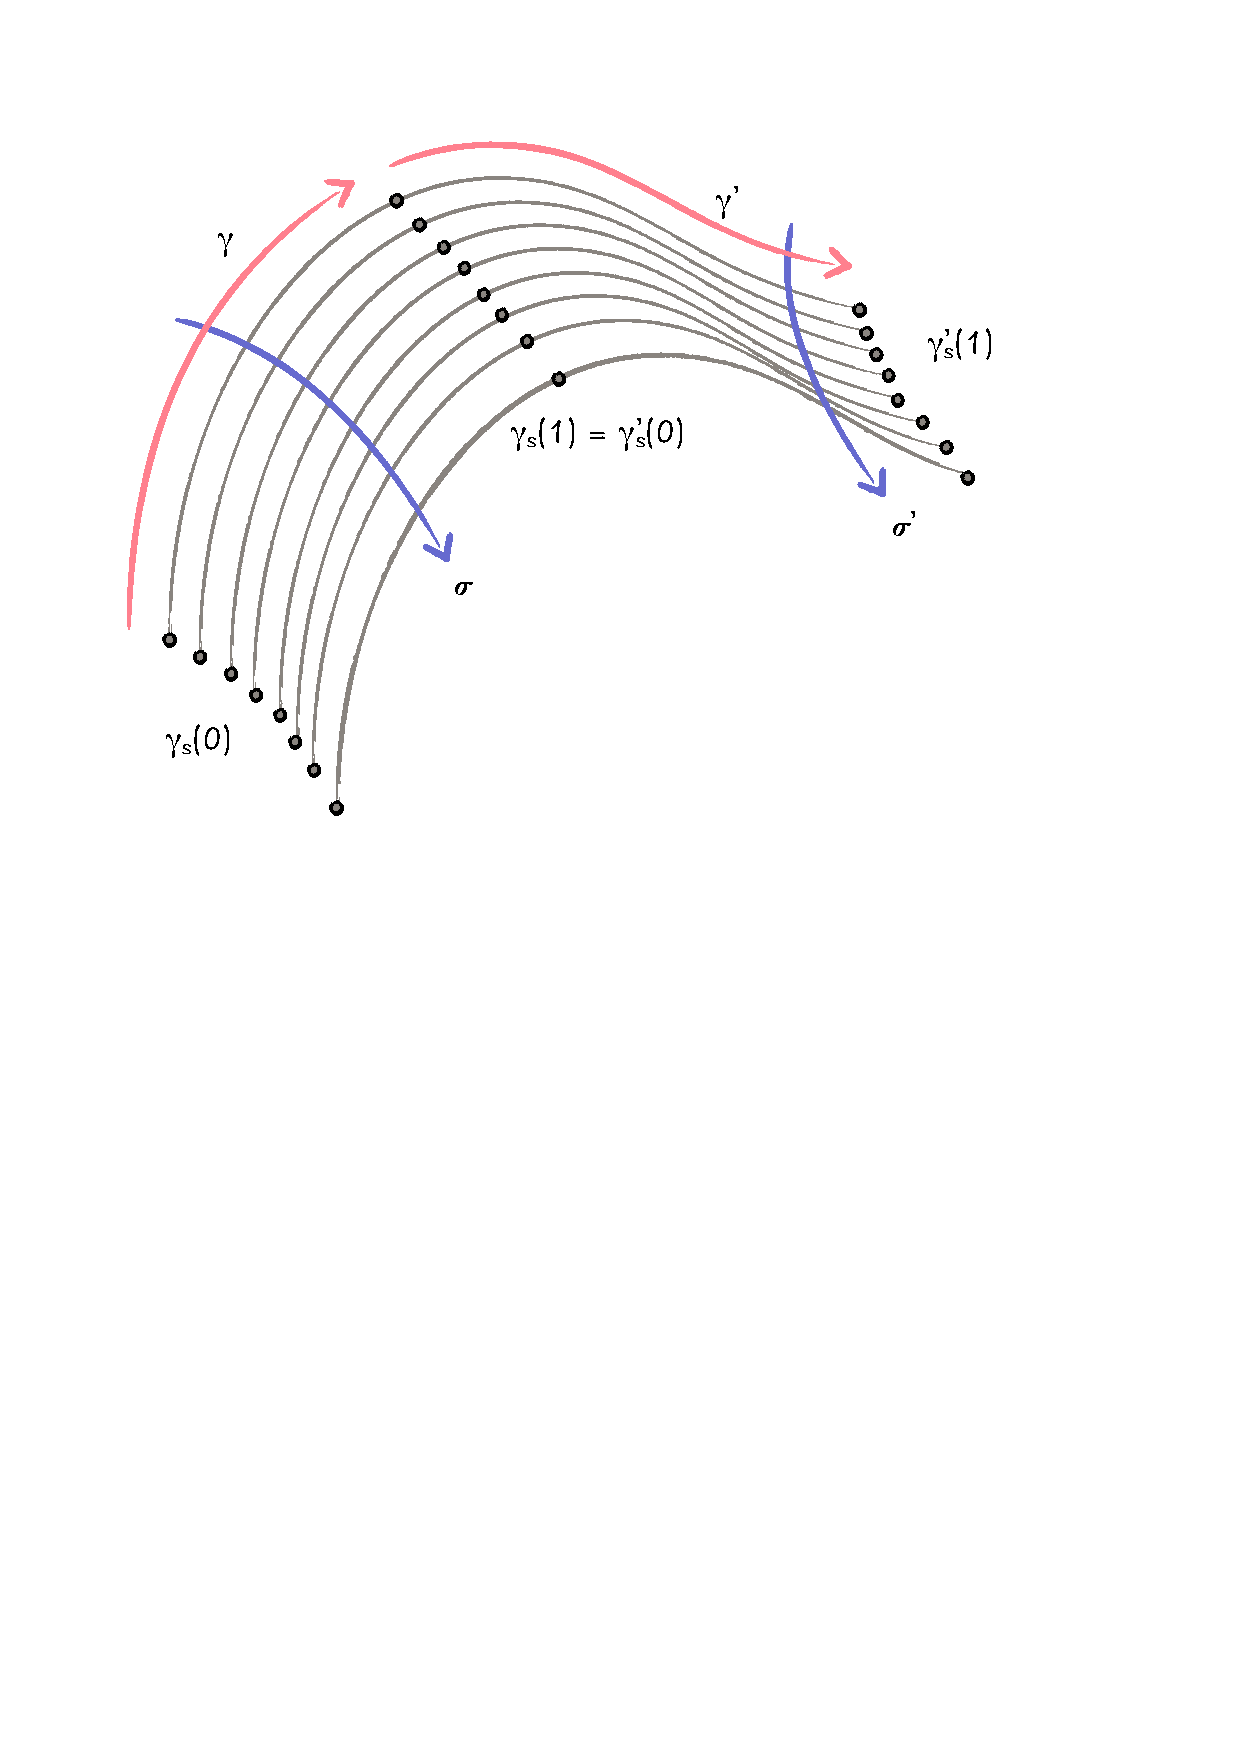
\includegraphics[width=.75\textwidth]{Figures/fig-concatenation-homotopy.pdf}
  \caption{Integrating concatenations over homotopies.}
  \label{fig:Integrating concatenations over homotopies}
\end{figure}

%%%%%%%%%%%%%%%%%%%%%%%%%%%%%%%%%%%%%%%%%%%%%%%%%%%%%%%%%%%
%% MARK:  Article — The Chasles Cocycle for a Closed 2-Form
%%%%%%%%%%%%%%%%%%%%%%%%%%%%%%%%%%%%%%%%%%%%%%%%%%%%%%%%%%%
\begin{article}\artlabel[The Chasles Cocycle for a Closed $2$-Form]
  \label{art:chases-cocycle-2form}
  
  We now assemble the local integration functions on the slices
  $\Paths(X,x,x')$ into a single global object.
  Consider the space of pairs of paths with common endpoints,
  introduced in the section header:
  \[
    \Paths_2(X) = \{ (\gamma,\gamma') \in \Paths(X) \times \Paths(X) \mid \EndsMap(\gamma) = \EndsMap(\gamma') \},
    \]%
  equipped with the subset diffeology of the product.
  The space $\Paths_2(X)$ is the fiber product of $\Paths(X)$ with itself over $X \times X$,
  denoted $\Paths(X) \times_{X \times X} \Paths(X)$.
  In categorical terms,
  it is the \emph{kernel pair} of the projection $\EndsMap$,
  acting as its self-pullback according to the following commutative diagram:
  
  \begin{center}
    \begin{tikzcd}[column sep=large, row sep=large, every label/.append style = {font = \small}]
      \Paths_2(X) = \EndsMap^*(\Paths(X)) \arrow[r,"\pr_2"] \arrow[d, swap, "\pr_1"] & \Paths(X) \arrow[d, "\EndsMap"]  \\
      \Paths(X) \arrow[r, swap, "\EndsMap"] & X \times X
    \end{tikzcd}
  \end{center}
  
  It projects over $X \times X$ via the map
  $(\gamma,\gamma') \mapsto \EndsMap(\gamma) = \EndsMap(\gamma')$,
  and the inverse-image over $(x,x')$ is precisely
  $\Paths(X,x,x') \times \Paths(X,x,x')$.
  
  \begin{proposition}[1]
    The space $\Paths_2(X)$ is homotopy equivalent to $\Loops(X)$.
    In particular,
    under the hypothesis that $X$ is simply connected,
    $\Paths_2(X)$ is connected.
  \end{proposition}
  
  Now consider the Action Form $\Komega$ on $\Paths(X)$.
  Pull it back to $\Paths_2(X)$ via the two canonical projections
  $\pr_1, \pr_2: \Paths_2(X) \to \Paths(X)$,
  where $\pr_1(\gamma,\gamma') = \gamma$ and $\pr_2(\gamma,\gamma') = \gamma'$.
  The difference
  \[
    \pr_1^*\Komega - \pr_2^*\Komega \in \DForms^1(\Paths_2(X))
    \]%
  is a closed $1$-form on $\Paths_2(X)$.
  Indeed,
  its exterior derivative is
  \[
    \der(\pr_1^*\Komega - \pr_2^*\Komega)
    = \pr_1^*(\der\Komega) - \pr_2^*(\der\Komega)
    = \pr_1^*(\1^*\omega - \0^*\omega) - \pr_2^*(\1^*\omega - \0^*\omega).
    \]%
  On $\Paths_2(X)$ we have $\0 \circ \pr_1 = \0 \circ \pr_2$ and
  $\1 \circ \pr_1 = \1 \circ \pr_2$,
  so the terms cancel and the form is closed.
  
  \begin{proposition}[2]
    The closed $1$-form $\pr_1^*\Komega - \pr_2^*\Komega$ on $\Paths_2(X)$
    has the same periods as the closed $1$-form
    $\Komega \restriction \Loops(X)$ on $\Loops(X)$.
  \end{proposition}
  
  Because $\Paths_2(X)$ is connected and carries a closed $1$-form
  whose period group is exactly $\Pomega$,
  the integration theorem for closed $1$-forms
  (Article~\ref{art: Integration of Closed 1-forms})
  applies directly.
  We obtain a smooth map
  \[
    \phi: \Paths_2(X) \to \Tomega,
    \]%
  unique up to an additive constant,
  satisfying
  \[
    \phi^*(\theta_\omega) = \pr_1^*\Komega - \pr_2^*\Komega,
    \]%
  where $\theta_\omega$ is the canonical $1$-form on $\Tomega$.
  
  \begin{definition}
    The map $\phi: \Paths_2(X) \to \Tomega$ is called the
    \emph{Chasles Cocycle} of the parasymplectic space $(X,\omega)$.
    We normalize it by requiring that
    $\phi(\gamma,\gamma) = 0$ for every path $\gamma \in \Paths(X)$.
  \end{definition}
  
  With this normalization,
  $\phi$ admits an explicit description.
  For any pair $(\gamma,\gamma') \in \Paths_2(X)$ with
  $\EndsMap(\gamma) = \EndsMap(\gamma') = (x,x')$,
  choose a path $\sigma$ in the slice $\Paths(X,x,x')$
  from $\gamma'$ to $\gamma$.
  Then
  \begin{equation}\tag{$\diamondsuit$}
    \phi(\gamma,\gamma') = \int_\sigma \Komega_{x,x'} \mod \Pomega.
  \end{equation}
  Equivalently,
  $\phi(\gamma,\gamma')$ is the projection to $\Tomega$ of the integral
  of the Action Form along any path in $\Paths(X,x,x')$
  connecting $\gamma'$ to $\gamma$.
  
  \begin{proposition}[3 --- Chasles Identity]
    The Chasles Cocycle satisfies the additive property
    \[
      \phi(\gamma,\gamma') + \phi(\gamma',\gamma'') = \phi(\gamma,\gamma''),
      \]%
    for any $\gamma,\gamma',\gamma'' \in \Paths(X)$ with
    $\EndsMap(\gamma) = \EndsMap(\gamma') = \EndsMap(\gamma'')$.
  \end{proposition}
  
  The Chasles Cocycle is the device that assembles the local integration
  functions $f_{x,x'}$ on each slice $\Paths(X,x,x')$
  into a single global object on $\Paths_2(X)$.
  Its cocycle property is the algebraic signature of the fact
  that the symplectic action is additive under concatenation of paths.
  In the next article,
  we will see how this cocycle defines an equivalence relation
  on the space of paths,
  and how the quotient by this relation yields the
  Prequantum Groupoid.
\end{article}

\begin{proof}
  Let us recall that $\Paths(X)$ and $\Loops(X)$ are homotopy equivalent to the spaces of strongly stationary paths and loops,
  see \cite[\textsection 5.5]{PIZ13}.
  Therefore,
  we work directly with stationary paths and loops without explicitly recalling this hypothesis at every step.
  
  \textbf{Homotopy equivalence.}~Let us begin by proving that $\Paths_2(X)$ is homotopy equivalent to $\Loops(X)$.
  We consider the subspace $\Loops_{1/2}(X)$ of loops that are stationary at $t = 1/2$,
  that is,
  constant on an open interval $\mathopen]1/2 -\varepsilon, 1/2+\varepsilon\mathclose[$.
  The proof in \cite[Ex. 84]{PIZ13} can be easily adapted to show that $\Loops(X)$ and $\Loops_{1/2}(X)$ are homotopy equivalent.
  Now,
  define the map
  \[
    \Phi: \Paths_2(X) \to \Loops_{1/2}(X),
    \qquad
    \Phi(\gamma,\gamma') = \gamma \vee \bar\gamma',
    \]
  where $\bar\gamma'$ is the reversed path $\bar\gamma'(t) = \gamma'(1-t)$.
  Next,
  define the reverse map
  \[
    \bar\Phi : \Loops_{1/2}(X) \to \Paths_2(X),
    \qquad
    \bar\Phi(\ell) = (\gamma,\gamma')
    \]
  with the components given by:
  \[
    \gamma(t) =
    \begin{cases}
    \ell(t/2) & \text{if } 0 \leq t \leq 1, \\
    \ell(0)   & \text{if } t \leq 0, \\
    \ell(1/2) & \text{if } t \geq 1,
    \end{cases}
    \qquad\text{and}\qquad
    \gamma'(t) =
    \begin{cases}
    \ell(1-t/2) & \text{if } 0 \leq t \leq 1, \\
    \ell(1)     & \text{if } t \leq 0, \\
    \ell(1/2)   & \text{if } t \geq 1.
    \end{cases}
    \]
  These two maps,
  $\Phi$ and $\bar\Phi$,
  are smooth and are homotopy inverses of each other.
  Therefore,
  $\Paths_2(X)$ is homotopy equivalent to $\Loops(X)$.
  
  Since $X$ is simply connected,
  $\pi_1(X,x) = \pi_0(\Loops(X,x)) = \{0\}$.
  Because $\pi_0(\Loops(X))$ is a quotient of $\pi_0(\Loops(X,x))$ \cite[Ex. 87]{PIZ13},
  it follows that $\Loops(X)$ is connected.
  Consequently,
  $\Paths_2(X)$ is also connected.
  
  \textbf{Pullback of $\Komega$ by $\Phi$.}~We now show that the map $\Phi$ satisfies the crucial identity:
  \[
    \Phi^*(\Komega \restriction \Loops(X)) = \pr_1^*(\Komega) - \pr_2^*(\Komega).
    \]
  Because a $1$-form in diffeology is entirely determined by its evaluation on $1$-plots \cite[\textsection 6.37]{PIZ13},
  it suffices to check this identity on paths.
  Let $s \mapsto (\gamma_s, \gamma'_s)$ be any $1$-plot (a smooth path) in $\Paths_2(X)$.
  Applying $\Phi$ yields the $1$-plot $s \mapsto \gamma_s \vee \bar\gamma'_s$ in $\Loops_{1/2}(X)$.
  By the additivity of $\Komega$ over concatenations of homotopies established in Article~\ref{art:Integrating Concatenations over Homotopies},
  we have:
  \[
    \Komega(s \mapsto \gamma_s \vee \bar\gamma'_s) = \Komega(s \mapsto \gamma_s) + \Komega(s \mapsto \bar\gamma'_s).
    \]
  By the change of integration parameter $t \mapsto 1-t$ in the definition of the chain-homotopy operator,
  reversing the path yields a minus sign:
  $\Komega(s \mapsto \bar\gamma'_s) = - \Komega(s \mapsto \gamma'_s)$.
  Therefore,
  evaluated on any $1$-plot,
  we find $\Phi^*(\Komega) = \pr_1^*(\Komega) - \pr_2^*(\Komega)$.
  Because $\Phi$ is a homotopy equivalence,
  it induces an isomorphism in de Rham cohomology \cite[\textsection 6.88]{PIZ13},
  ensuring that the $1$-form $\pr_1^*(\Komega) - \pr_2^*(\Komega)$ shares the exact same periods $\Pomega$ as $\Komega \restriction \Loops(X)$.
  
  \textbf{The Function $\pmb{\phi}$.}~We have assumed that the periods $\Pomega$ of $\Komega \restriction \Loops(X)$ form a strict subgroup of $\RR$,
  and are therefore discrete in the diffeological sense.
  Since $\Loops(X)$ is connected,
  let $f \in \Cinfty(\Loops(X),\Tomega)$ be the integration function (Article \ref{art: Integration of Closed 1-forms}) normalized such that $f(\hat{x}) = 0$,
  where $\hat{x}$ is the constant loop at $x$.
  It satisfies $f^*(\theta_\omega) = \Komega \restriction \Loops(X)$.
  
  We define the Chasles cocycle by pulling back this integration function:
  \[
    \phi = f \circ \Phi \in \Cinfty(\Paths_2(X), \Tomega).
    \]
  This construction automatically guarantees that
  \[
    \phi^*(\theta_\omega) = \Phi^*(f^*(\theta_\omega)) = \Phi^*(\Komega) = \pr_1^*(\Komega) - \pr_2^*(\Komega).
    \]
  Furthermore,
  because $\Phi(\gamma,\gamma) = \gamma \vee \bar\gamma$,
  which is canonically homotopic to the constant loop $\hat{x}$,
  our normalization ensures $\phi(\gamma,\gamma) = 0$.
  
  We now verify the explicit formula ($\diamondsuit$).
  Fix a pair $(\gamma, \gamma') \in \Paths_2(X)$ with endpoints $(x,x')$.
  By definition of $f$,
  we have:
  \[
    \phi(\gamma,\gamma') = f(\gamma \vee \bar\gamma') = \int_{\hat{x}}^{\gamma \vee \bar\gamma'} \Komega \restriction \Loops(X,x) \mod \Pomega,
    \]
  where the integral is computed along any smooth path in $\Loops(X,x)$ connecting the constant loop $\hat{x}$ to $\gamma \vee \bar\gamma'$.
  
  Let $\sigma : s \mapsto \eta_s$ be a path in the slice $\Paths(X,x,x')$ from $\gamma'$ to $\gamma$.
  Consider the smooth map
  \[
    \nu : \Paths(X,x,x') \to \Loops(X,x),
    \qquad
    \nu(\eta) = \gamma \vee \bar\eta.
    \]
  \textbf{Lemma.}~ We have $\nu^*(\Komega \restriction \Loops(X,x)) = - \Komega_{x,x'}$.
  
  \textit{Proof of Lemma.}~Applying the concatenation identity from Article~\ref{art:Integrating Concatenations over Homotopies} to the constant plot $s \mapsto \gamma$ and the varying plot $s \mapsto \bar\eta_s$,
  we evaluate the form on the $1$-plot $s \mapsto \eta_s$:
  \[
    \nu^*(\Komega)(s \mapsto \eta_s) = \Komega(s \mapsto \gamma \vee \bar\eta_s) = \Komega(s \mapsto \gamma) + \Komega(s \mapsto \bar\eta_s).
    \]
  Since $s \mapsto \gamma$ is constant,
  its variation is zero,
  so the first term vanishes.
  The second term yields $- \Komega(s \mapsto \eta_s)$.
  Thus,
  evaluated on any $1$-plot,
  the forms are equal. \hfill$\square$
  
  We now apply the invariance of integration on chains \cite[\textsection 6.67]{PIZ13}.
  The pushed-forward path $\nu \circ \sigma$ in $\Loops(X,x)$ runs from $\nu(\gamma') = \gamma \vee \bar\gamma'$ to $\nu(\gamma) = \gamma \vee \bar\gamma$.
  Therefore:
  \[
    \int_{\nu \circ \sigma} \Komega \restriction \Loops(X,x) = \int_\sigma \nu^*(\Komega \restriction \Loops(X,x)) = - \int_\sigma \Komega_{x,x'} = - \int_{\gamma'}^\gamma \Komega_{x,x'}.
    \]
  On the other hand,
  evaluating the integral directly in $\Loops(X,x)$ yields:
  \begin{align*}
  %\int_{\nu \circ \sigma} \Komega = \int_{\gamma \vee \bar\gamma'}^{\gamma \vee \bar\gamma} \Komega & = \underbrace{\int_{\gamma \vee \bar\gamma'}^{\hat{x}} \Komega}_{\displaystyle = - \int_{\hat{x}}^{\gamma \vee \bar\gamma'} \Komega} + \underbrace{\int_{\hat{x}}^{\gamma \vee \bar\gamma} \Komega}_{\displaystyle = 0}.
  \int_{\nu \circ \sigma} \Komega = \int_{\gamma \vee \bar\gamma'}^{\gamma \vee \bar\gamma} \Komega & = \int_{\gamma \vee \bar\gamma'}^{\hat{x}} \Komega + \int_{\hat{x}}^{\gamma \vee \bar\gamma} \Komega \\
  &  = - \int_{\hat{x}}^{\gamma \vee \bar\gamma'} \Komega + 0
\end{align*}
Equating the two results gives:
\[
  - \int_{\hat{x}}^{\gamma \vee \bar\gamma'} \Komega = - \int_{\gamma'}^\gamma \Komega_{x,x'}.
  \]
Projecting this identity modulo the periods $\Pomega$ confirms the formula ($\diamondsuit$):
$\phi(\gamma,\gamma') = \int_{\gamma'}^\gamma \Komega_{x,x'} \pmod \Pomega$.

\textbf{The Additive Cocycle Property.}~With the explicit formula established,
the Chasles identity becomes a trivial consequence of the additivity of the standard integral.
For any triple of paths $\gamma, \gamma', \gamma''$ sharing the same endpoints $(x,x')$,
we have:
\begin{align*}
  \phi(\gamma,\gamma') + \phi(\gamma',\gamma'') &= \left( \int_{\gamma'}^{\gamma} \Komega_{x,x'} + \int_{\gamma''}^{\gamma'} \Komega_{x,x'} \right) \mod \Pomega \\
  &= \int_{\gamma''}^{\gamma} \Komega_{x,x'} \mod \Pomega \\
  &= \phi(\gamma,\gamma'').
\end{align*}
This completes the proof.
\end{proof}

%%%%%%%%%%%%%%%%%%%%%%%%%%%%%%%%%%%%%%%%%%%%%%%%%%%%%%%%%%%
%% MARK:  Article — The Equivalence Relation $\sim_\omega$
%%%%%%%%%%%%%%%%%%%%%%%%%%%%%%%%%%%%%%%%%%%%%%%%%%%%%%%%%%%
\begin{article}\artlabel[The Equivalence Relation $\sim_\omega$]
  \label{art:equivalence-relation}
  The Chasles Cocycle $\phi: \Paths_2(X) \to \Tomega$ constructed in the
  previous article defines an equivalence relation on the space of paths.
  
  \begin{definition}
    Two paths $\gamma, \gamma' \in \Paths(X)$ are \emph{equivalent},
    denoted $\gamma \sim_\omega \gamma'$,
    if and only if they have the same endpoints and their relative
    symplectic action vanishes modulo the periods:
    \[
      \gamma \sim_\omega \gamma'
      \qtext{\Iff}
      \EndsMap(\gamma) = \EndsMap(\gamma')
      \qtext{and}
      \phi(\gamma,\gamma') = 0.
      \]
  \end{definition}
  
  Using the explicit formula ($\diamondsuit$) for $\phi$ established in
  Article~\ref{art:chases-cocycle-2form},
  the condition $\phi(\gamma,\gamma') = 0$ admits an equivalent
  formulation.
  Let $(x,x') = \EndsMap(\gamma) = \EndsMap(\gamma')$.
  Under our hypothesis that $X$ is simply connected, the slice of paths
  $\Paths(X,x,x')$ is connected (Primer, \S\ref{sec:Paths and Space of Paths}).
  Thus, there always exists a fixed-ends path $\sigma$ in the slice
  from $\gamma'$ to $\gamma$, and
  \[
    \gamma \sim_\omega \gamma'
    \qtext{\Iff}
    \EndsMap(\gamma) = \EndsMap(\gamma')
    \qtext{and}
    \int_{\gamma'}^\gamma \Komega_{x,x'} \in \Pomega.
    \]
  In words,
  two paths are equivalent if they share the same endpoints
  and the integral of the Action Form along any homotopy between them
  belongs to the Group of Periods.
  
  The choice of homotopy $\sigma$ is completely irrelevant.
  Indeed, if $\sigma_1$ and $\sigma_2$ are two homotopies from $\gamma'$ to $\gamma$ in $\Paths(X,x,x')$,
  their concatenation $\sigma_1 \vee \bar{\sigma}_2$ is a loop of paths,
  which evaluates to a period in $\Pomega$ (Article~\ref{art:group-of-periods}).
  Consequently:
  \[
    \int_{\sigma_1} \Komega_{x,x'} - \int_{\sigma_2} \Komega_{x,x'} = \int_{\sigma_1 \vee \bar{\sigma}_2} \Komega \in \Pomega.
    \]
\end{article}

\begin{proof}
  We verify that the relation $\sim_\omega$ satisfies the axioms of an equivalence relation.
  
  \textbf{Reflexivity.}
  For any path $\gamma \in \Paths(X)$,
  the normalization of the Chasles cocycle gives $\phi(\gamma,\gamma) = 0$.
  Thus, $\gamma \sim_\omega \gamma$.
  
  \textbf{Symmetry.}
  Assume $\gamma \sim_\omega \gamma'$, so $\EndsMap(\gamma) = \EndsMap(\gamma')$ and $\phi(\gamma,\gamma') = 0$.
  Applying the Chasles identity (Article~\ref{art:chases-cocycle-2form}, Prop. 3) to the triple $(\gamma', \gamma, \gamma')$ yields:
  \[
    \phi(\gamma',\gamma) + \phi(\gamma,\gamma') = \phi(\gamma',\gamma') = 0.
    \]
  Since $\phi(\gamma,\gamma') = 0$, we immediately obtain $\phi(\gamma',\gamma) = 0$.
  Therefore, $\gamma' \sim_\omega \gamma$.
  
  \textbf{Transitivity.}
  Assume $\gamma \sim_\omega \gamma'$ and $\gamma' \sim_\omega \gamma''$.
  Thus, we have $\EndsMap(\gamma) = \EndsMap(\gamma') = \EndsMap(\gamma'')$, as well as $\phi(\gamma,\gamma') = 0$ and $\phi(\gamma',\gamma'') = 0$.
  The additive property of the Chasles identity yields:
  \[
    \phi(\gamma,\gamma'') = \phi(\gamma,\gamma') + \phi(\gamma',\gamma'') = 0 + 0 = 0.
    \]
  Since the endpoints also match, we conclude $\gamma \sim_\omega \gamma''$.
\end{proof}

%%%%%%%%%%%%%%%%%%%%%%%%%%%%%%%%%%%%%%%%%%%%%%%%%%%%%%%%%%%
%%
%% MARK: Section — Construction of the Quantum System
%%
%%%%%%%%%%%%%%%%%%%%%%%%%%%%%%%%%%%%%%%%%%%%%%%%%%%%%%%%%%%
\section{Construction of the Quantum System}
\label{sec:Construction of the Quantum System}

%%%%%%%%%%%%%%%%%%%%%%%%%%%%%%%%%%%%%%%%%%%%%%%%%%%%%%%%%%%
%% MARK:  Article —
%%%%%%%%%%%%%%%%%%%%%%%%%%%%%%%%%%%%%%%%%%%%%%%%%%%%%%%%%%%
\begin{article}\artlabel[Statement of the Main Theorem]
  \label{art:main-theorem-statement}
  ...
\end{article}

%%%%%%%%%%%%%%%%%%%%%%%%%%%%%%%%%%%%%%%%%%%%%%%%%%%%%%%%%%%
%% MARK:  Article —
%%%%%%%%%%%%%%%%%%%%%%%%%%%%%%%%%%%%%%%%%%%%%%%%%%%%%%%%%%%
\begin{article}\artlabel[The Groupoid $\Groupoid{T}_\omega$]
  \label{art:groupoid-construction}
  ...
\end{article}

%%%%%%%%%%%%%%%%%%%%%%%%%%%%%%%%%%%%%%%%%%%%%%%%%%%%%%%%%%%
%%
%% MARK: Section — The Prequantum 1-Form and its Curvature
%%
%%%%%%%%%%%%%%%%%%%%%%%%%%%%%%%%%%%%%%%%%%%%%%%%%%%%%%%%%%%
\section{The Prequantum $1$-Form and its Curvature}
\label{sec:The Prequantum 1-Form and its Curvature}

%%%%%%%%%%%%%%%%%%%%%%%%%%%%%%%%%%%%%%%%%%%%%%%%%%%%%%%%%%%
%% MARK:  Article —
%%%%%%%%%%%%%%%%%%%%%%%%%%%%%%%%%%%%%%%%%%%%%%%%%%%%%%%%%%%
\begin{article}\artlabel[Existence, Uniqueness, and Invariance of $\blambda$]
  \label{art:existence-prequantum-form}
  ...
\end{article}

%%%%%%%%%%%%%%%%%%%%%%%%%%%%%%%%%%%%%%%%%%%%%%%%%%%%%%%%%%%
%% MARK:  Article —
%%%%%%%%%%%%%%%%%%%%%%%%%%%%%%%%%%%%%%%%%%%%%%%%%%%%%%%%%%%
\begin{article}\artlabel[Curvature of the Prequantum $1$-Form]
  \label{art:curvature-prequantum-form}
  ...
\end{article}

%%%%%%%%%%%%%%%%%%%%%%%%%%%%%%%%%%%%%%%%%%%%%%%%%%%%%%%%%%%
%%
%% MARK: Section — The Isotropy Group as the Torus of Periods
%%
%%%%%%%%%%%%%%%%%%%%%%%%%%%%%%%%%%%%%%%%%%%%%%%%%%%%%%%%%%%
\section{The Isotropy Group as the Torus of Periods}
\label{sec:The Isotropy Group as the Torus of Periods}

%%%%%%%%%%%%%%%%%%%%%%%%%%%%%%%%%%%%%%%%%%%%%%%%%%%%%%%%%%%
%% MARK:  Article —
%%%%%%%%%%%%%%%%%%%%%%%%%%%%%%%%%%%%%%%%%%%%%%%%%%%%%%%%%%%
\begin{article}\artlabel[The Isotropy Group $\Groupoid{T}_{\omega,x}$]
  \label{art:isotropy-statement}
  ...
\end{article}

%%%%%%%%%%%%%%%%%%%%%%%%%%%%%%%%%%%%%%%%%%%%%%%%%%%%%%%%%%%
%% MARK:  Article —
%%%%%%%%%%%%%%%%%%%%%%%%%%%%%%%%%%%%%%%%%%%%%%%%%%%%%%%%%%%
\begin{article}\artlabel[Proof that the Isotropy Isomorphism is a Subduction]
  \label{art:isotropy-subduction}
  ...
\end{article}

%%%%%%%%%%%%%%%%%%%%%%%%%%%%%%%%%%%%%%%%%%%%%%%%%%%%%%%%%%%
%%
%% MARK: Section — The Full and Faithful Representation of Symmetries
%%
%%%%%%%%%%%%%%%%%%%%%%%%%%%%%%%%%%%%%%%%%%%%%%%%%%%%%%%%%%%
\section{The Full and Faithful Representation of Symmetries}
\label{sec:The Full and Faithful Representation of Symmetries}

%%%%%%%%%%%%%%%%%%%%%%%%%%%%%%%%%%%%%%%%%%%%%%%%%%%%%%%%%%%
%% MARK:  Article —
%%%%%%%%%%%%%%%%%%%%%%%%%%%%%%%%%%%%%%%%%%%%%%%%%%%%%%%%%%%
\begin{article}\artlabel[Lift of Classical Symmetries to the Groupoid]
  \label{art:lift-symmetries}
  ...
\end{article}

%%%%%%%%%%%%%%%%%%%%%%%%%%%%%%%%%%%%%%%%%%%%%%%%%%%%%%%%%%%
%% MARK:  Article —
%%%%%%%%%%%%%%%%%%%%%%%%%%%%%%%%%%%%%%%%%%%%%%%%%%%%%%%%%%%
\begin{article}\artlabel[The Isomorphism $\Aut(\Groupoid{T}_\omega,\blambda) \simeq \Diff(X,\omega)$]
  \label{art:automorphism-isomorphism}
  ...
\end{article}

%%%%%%%%%%%%%%%%%%%%%%%%%%%%%%%%%%%%%%%%%%%%%%%%%%%%%%%%%%%
%% MARK:  Article —
%%%%%%%%%%%%%%%%%%%%%%%%%%%%%%%%%%%%%%%%%%%%%%%%%%%%%%%%%%%
\begin{article}\artlabel[Why Central Extensions Do Not Appear at the Groupoid Level]
  \label{art:no-central-extensions}
  ...
\end{article}
